\chapter{Reference Data Tables}
\label{app:data}

This appendix collects the numerical scales used throughout the monograph: ranges of $n_{\mathrm{e}}$, $n_{\mathrm{i}}$, $T_{\mathrm{e}}$, and $T_{\mathrm{i}}$ for the three application domains; sputter-yield thresholds; ion-energy and sheath-potential scales; and reference Debye lengths $\lambda_{\mathrm{D}}$ and Bohm velocities $u_{\mathrm{B}}$ for common gases. Entries are closed-form evaluations of expressions derived in Chapters~2--4, or literature-compiled figures labelled as such; none is an original measurement.

\section{Typical Plasma Parameter Ranges for the Three Application Domains}
\label{app:data:domains}

The main text motivates the ion-energy-flux formalism with three domains sharing the same sheath physics but occupying very different parameter regions: low-temperature RF processing, the magnetically confined fusion boundary (scrape-off layer and divertor), and electric propulsion. Table~\ref{tab:domains} summarises characteristic density, temperatures, magnetic field, pressure, and species for each; values are orientation, not strict bounds.

\begin{table}[htbp]
\centering
\caption{Representative operating ranges of key plasma parameters in the three application domains treated in this monograph. Values are order-of-magnitude, literature-representative ranges, not measurements from this work.}
\label{tab:domains}
\begin{tabularx}{\textwidth}{@{}l X X X@{}}
\toprule
Parameter & RF processing plasma & Fusion edge / divertor & Electric propulsion \\
\midrule
$n_{\mathrm{e}}$ & \SI{1e15}{} -- \SI{1e18}{\per\cubic\meter} & \SI{1e18}{} -- \SI{1e21}{\per\cubic\meter} & \SI{1e15}{} -- \SI{1e19}{\per\cubic\meter} \\
$T_{\mathrm{e}}$ & \SI{1}{} -- \SI{7}{\eV} & \SI{1}{} -- \SI{100}{\eV} & \SI{1}{} -- \SI{30}{\eV} \\
$T_{\mathrm{i}}$ & \SI{0.03}{} -- \SI{0.5}{\eV} & comparable to $T_{\mathrm{e}}$, up to a few $T_{\mathrm{e}}$ & \SI{0.1}{} -- \SI{5}{\eV} (directed beam spread) \\
Magnetic field $B$ & $0$ -- few \si{\milli\tesla} (magnetised ICP) & \SI{1}{} -- \SI{8}{\tesla} & \SI{1}{} -- \SI{20}{\milli\tesla} (radial, Hall channel) \\
Neutral pressure & \SI{0.1}{} -- \SI{13}{\pascal} & effectively vacuum in confined region & \SI{1e-3}{} -- \SI{1}{\pascal} \\
Typical species & Ar, O$_2$, N$_2$, Cl$_2$, SF$_6$ & D, T, He, seeded N/Ne/Ar & Xe, Kr, occasionally I$_2$, Ar \\
\bottomrule
\end{tabularx}
\end{table}

Three features recur. First, $T_{\mathrm{e}}$ stays within a narrow band, $\SI{1}{\eV} \lesssim T_{\mathrm{e}} \lesssim \SI{100}{\eV}$, fixed by the atomic physics of ionisation that sustains a discharge. Second, $n_{\mathrm{e}}$ spans many orders of magnitude, from tenuous thruster plumes to dense divertor plasma, and together with $T_{\mathrm{e}}$ sets the Debye length and sheath thickness (Section~\ref{app:data:debye}). Third, in RF processing and electric-propulsion plasmas $T_{\mathrm{i}} \ll T_{\mathrm{e}}$, an ordering that makes the Bohm criterion tractable \cite{ref0001,ref0013}; in the fusion edge, however, $T_{\mathrm{i}}$ can be comparable to, or a few times, $T_{\mathrm{e}}$, requiring the warm-ion Bohm generalisation discussed in Section~\ref{app:data:energy}.

In the fusion edge, the wide range reflects the transition from the hot upstream SOL to the cold, dense, often detached divertor target \cite{ref0013,ref0017}. In electric propulsion, it reflects the dense, magnetised discharge channel versus the far more tenuous plume; ion energy and flux there underpin erosion and lifetime assessments \cite{ref0074,ref0105}.

\section{Representative Sputter-Yield Thresholds and Trends by Material}
\label{app:data:sputter}

Physical sputtering is the ejection of a surface atom by momentum transferred from an incident ion through a collision cascade, underlying erosion of plasma-facing components, thruster grids, and processing-chamber walls. The key quantity is the sputter yield $Y(E,\theta)$, the mean number of atoms ejected per incident ion of energy $E$ and angle $\theta$. At normal incidence the yield is strongly threshold-like: below $E_{\mathrm{th}}$ the ion cannot overcome the surface binding energy $U_0$ and $Y \to 0$; above threshold $Y$ rises, peaks broadly in the \si{\kilo\eV} range, then falls as the ion penetrates too deeply for the cascade to reach the surface \cite{ref0143,ref0144}.

A widely used empirical parameterisation, due to Bohdansky and refined by Yamamura, writes the yield as a nuclear-stopping cross-section times a threshold factor,
\begin{equation}
Y(E) = Q \, S_{n}(E) \left[1 - \left(\frac{E_{\mathrm{th}}}{E}\right)^{2/3}\right]\left[1 - \frac{E_{\mathrm{th}}}{E}\right]^{2},
\qquad E \geq E_{\mathrm{th}},
\label{appD-eq:bohdansky}
\end{equation}
and $Y(E)=0$ for $E<E_{\mathrm{th}}$, where $Q$ is a material-dependent factor and $S_n(E)$ the reduced nuclear stopping cross-section \cite{ref0144}. The threshold requires the ion to impart energy of order $U_0$ to a target atom in one close collision, giving
\begin{equation}
E_{\mathrm{th}} \approx
\begin{cases}
U_0/[\gamma(1-\gamma)], & M_{\mathrm{i}}/M_{\mathrm{t}} \lesssim 0.3, \\[2pt]
8\,U_0\,(M_{\mathrm{i}}/M_{\mathrm{t}})^{2/5}, & M_{\mathrm{i}}/M_{\mathrm{t}} \gtrsim 0.3,
\end{cases}
\qquad
\gamma = \frac{4 M_{\mathrm{i}} M_{\mathrm{t}}}{(M_{\mathrm{i}}+M_{\mathrm{t}})^{2}},
\label{eq:ethresh}
\end{equation}
with $M_{\mathrm{i}}$, $M_{\mathrm{t}}$ the ion and target masses and $\gamma$ the maximum fractional energy transfer per collision; the first (light-ion) branch applies for mass ratio $M_{\mathrm{i}}/M_{\mathrm{t}} \lesssim 0.3$, the second (near-unity mass ratio) branch otherwise. Light ions (H, D, He) sputter heavy targets (W, Mo) weakly, above a high threshold, since mass mismatch makes $\gamma$ small, while mass-matched pairs (e.g.\ Ar$^+$ on Cu) couple efficiently at low threshold via the second branch.

Table~\ref{tab:sputter} lists representative threshold energies and a reference yield for materials relevant to fusion plasma-facing components and processing. These are order-of-magnitude values: measured yields depend on species, angle, roughness, temperature, and fluence, and can vary by a factor of two between sources \cite{ref0152,ref0158}.

\begin{table}[htbp]
\centering
\caption{Representative (literature-typical) sputter-yield thresholds and reference yields for selected target materials. Values are order-of-magnitude figures compiled from the classical sputtering-yield literature and are \emph{not} measurements from this work; actual yields depend on ion species, angle, surface condition, and fluence.}
\label{tab:sputter}
\begin{tabular}{@{}llccl@{}}
\toprule
Target & Bombarding ion & $E_{\mathrm{th}}$ [\si{\eV}] & $Y$ at \SI{500}{\eV} & Remarks \\
\midrule
W & D$^{+}$ & $\sim 200$--230 & $\sim 10^{-3}$--$10^{-2}$ & high threshold; dominant divertor concern \cite{ref0158} \\
W & He$^{+}$ & $\sim 100$ & $\sim 10^{-2}$--$10^{-1}$ & enhanced by surface nanostructuring \\
W & Ar$^{+}$ & $\sim 30$ & $\sim 0.5$--1 & self-consistent heavy-ion benchmark \\
C (graphite) & D$^{+}$ & $\sim 35$--40 & $\sim 10^{-2}$ (physical only) & chemical erosion dominates below threshold \\
Be & D$^{+}$ & $\sim 10$--15 & $\sim 10^{-2}$--$10^{-1}$ & low threshold; ITER first-wall relevance \\
Mo & Ar$^{+}$ & $\sim 25$ & $\sim 0.7$--1 & alternative divertor material \\
Cu & Ar$^{+}$ & $\sim 17$--20 & $\sim 2$--2.5 & reference material for yield benchmarking \\
Si & Ar$^{+}$ & $\sim 20$ & $\sim 0.5$--0.8 & processing/etch-mask relevance \\
Stainless steel & Ar$^{+}$ & $\sim 20$--25 & $\sim 1$--1.5 & representative of chamber-wall erosion \\
\bottomrule
\end{tabular}
\end{table}

This trend -- light-on-heavy pairs give high threshold and low yield, mass-matched pairs sputter efficiently at low threshold -- follows directly from $\gamma$ in Equation~\eqref{eq:ethresh}, and explains why fusion devices favour D/T fuelling against tungsten walls while accepting more efficient helium-ash erosion \cite{ref0143}. Realistic multi-species bombardment also shows synergistic effects not captured by Equation~\eqref{appD-eq:bohdansky} alone.

Figure~\ref{fig:yield} shows the qualitative shape of Equation~\eqref{appD-eq:bohdansky}, via the bracketed threshold factor
\begin{equation}
\hat{Y}(x) = \left(1-x^{-2/3}\right)\left(1-x^{-1}\right)^{2}, \qquad x \equiv E/E_{\mathrm{th}} \geq 1,
\label{eq:yieldnorm}
\end{equation}
versus reduced energy $x$; it excludes $S_n(E)$ and is not an absolute yield curve for any material.

\begin{figure}[htbp]
\centering
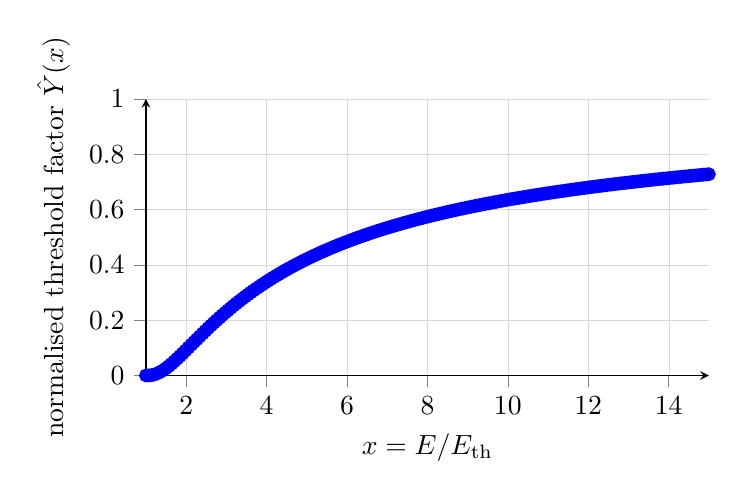
\begin{tikzpicture}
\begin{axis}[
 width=0.72\textwidth,
 height=0.42\textwidth,
 xlabel={$x = E/E_{\mathrm{th}}$},
 ylabel={normalised threshold factor $\hat{Y}(x)$},
 xmin=1, xmax=15,
 ymin=0, ymax=1,
 domain=1:15,
 samples=200,
 axis lines=left,
 tick align=outside,
 grid=major,
 grid style={line width=0.1pt, draw=gray!30},
 every axis plot/.append style={line width=1pt, color=black},
]
\addplot {(1-x^(-2/3))*(1-x^(-1))^2};
\end{axis}
\end{tikzpicture}
\caption{Schematic, dimensionless illustration of the threshold factor $\hat Y(x)$ in the Bohdansky-type sputtering yield model of Equation~\eqref{eq:yieldnorm}, plotted as an explicit analytic function of the reduced energy $x=E/E_{\mathrm{th}}$. This is a mathematical illustration of the model's threshold shape only; it does not represent measured or material-specific yield data.}
\label{fig:yield}
\end{figure}

\section{Ion-Energy and Sheath-Potential Scales}
\label{app:data:energy}

Ion impact energy is set, to leading order, by the potential drop across the sheath, modified by the ion's kinetic energy at the sheath edge (fixed by the Bohm criterion) and, in time-varying sheaths, by transit-time dynamics. This section collects the relations converting a sheath potential into an ion energy flux $\Gamma_E$ at the wall.

\subsection{The Bohm criterion and the presheath potential drop}

A collisionless, quasineutral plasma supports a monotonic potential drop into a sheath only if ions enter the sheath edge at directed speed at or above the Bohm velocity $u_{\mathrm{B}}$,
\begin{equation}
u_{\mathrm{i}}(s) \geq u_{\mathrm{B}} \equiv \sqrt{\frac{k_{\mathrm{B}} T_{\mathrm{e}}}{M}} ,
\label{eq:bohmcrit}
\end{equation}
where $s$ is the sheath edge and $M$ the ion mass; its generalisations (finite $T_{\mathrm{i}}$, collisions, multiple species, magnetisation) form an extensive literature \cite{ref0001,ref0017}. Momentum balance in the presheath, where ions accelerate from bulk thermal speed to $u_{\mathrm{B}}$, requires a drop of order
\begin{equation}
\Delta \phi_{\mathrm{pre}} \sim \frac{1}{2}\,\frac{T_{\mathrm{e}}}{e},
\label{eq:presheath}
\end{equation}
independent, to leading order, of the transport mechanism (collisional friction, geometric divergence, ionisation) \cite{ref0013}. This minimum energy is acquired before the sheath proper, ahead of the typically larger sheath-potential acceleration.

\subsection{The floating potential and the mean bombardment energy}

For a floating, non-emitting surface, zero net current fixes the sheath drop $V_{\mathrm{sh}} = \phi_{\mathrm{s}} - \phi_{\mathrm{w}}$:
\begin{equation}
V_{\mathrm{f}} = \frac{T_{\mathrm{e}}}{2e}\ln\!\left[\frac{M}{2\pi m_{\mathrm{e}}}\right],
\label{eq:floating}
\end{equation}
obtained by equating the Bohm ion flux $n_{\mathrm{s}} u_{\mathrm{B}}$ to the thermal electron flux $\tfrac{1}{4} n_{\mathrm{s}} \bar v_{\mathrm{e}} \exp(-eV_{\mathrm{f}}/T_{\mathrm{e}})$, with $\bar v_{\mathrm{e}} = \sqrt{8 T_{\mathrm{e}}/\pi m_{\mathrm{e}}}$. Since $M/m_{\mathrm{e}}\sim10^{3}$--$10^{5}$, the logarithm is a modest factor, and
\begin{equation}
e V_{\mathrm{f}} \approx (3\text{--}6)\, T_{\mathrm{e}},
\end{equation}
the coefficient depending logarithmically on mass ratio and $T_{\mathrm{i}}/T_{\mathrm{e}}$. On an actively biased surface the drop is set externally, from a few volts to several kilovolts, with ion energy following the instantaneous or time-averaged potential depending on transit time \cite{ref0080,ref0105}.

In the collisionless limit, the mean bombardment energy is
\begin{equation}
\langle E_{\mathrm{i}} \rangle \approx e V_{\mathrm{sh}} + \frac{1}{2}M u_{\mathrm{B}}^{2} + \tfrac{1}{2}T_{\mathrm{i}}
\;=\; e V_{\mathrm{sh}} + \tfrac{1}{2}T_{\mathrm{e}} + \tfrac{1}{2}T_{\mathrm{i}},
\label{eq:meanenergy}
\end{equation}
where the last two terms are minor once bias exceeds a few tens of volts but dominate on an unbiased floating wall. Charge-exchange collisions broaden the distribution about $\langle E_{\mathrm{i}}\rangle$, producing the low-energy tail quantified by $f_{\mathrm{i}}(v)$ below \cite{ref0077}.

\subsection{Ion energy distribution and energy flux}

The ion energy flux to the surface:
\begin{equation}
\Gamma_{E} = \int_{0}^{\infty} \left(\tfrac{1}{2} M v^{2}\right) v\, f_{\mathrm{i}}(v)\, \mathrm{d}v
= \Gamma_{\mathrm{i}} \, \langle E_{\mathrm{i}} \rangle,
\qquad
\Gamma_{\mathrm{i}} = \int_{0}^{\infty} v\, f_{\mathrm{i}}(v)\, \mathrm{d}v = n_{\mathrm{s}} u_{\mathrm{B}},
\label{eq:energyflux}
\end{equation}
where $f_{\mathrm{i}}(v)$ is the wall ion distribution, normalised so $\int_0^\infty f_{\mathrm{i}}(v)\,\mathrm{d}v = n_{\mathrm{s}}$, and $\Gamma_{\mathrm{i}}$ is the particle flux fixed by the Bohm criterion to $n_{\mathrm{s}} u_{\mathrm{B}}$ \cite{ref0074,ref0090,ref0093}. This links to Section~\ref{app:data:sputter}: it is $\Gamma_E$, not $\Gamma_{\mathrm{i}}$ alone, that sets erosion or heat load once folded against a yield $Y(E)$, via $\Gamma_{\mathrm{erosion}} = \int Y(E)\, v\, f_{\mathrm{i}}(v)\, \mathrm{d}v$.

In a time-independent, near-collisionless sheath, $f_{\mathrm{i}}(v)$ collapses toward a narrow distribution centred on Equation~\eqref{eq:meanenergy}. In an RF-driven or pulsed sheath, finite transit time instead broadens $f_{\mathrm{i}}(v)$ into the bimodal or saddle-shaped distribution reported for capacitively coupled discharges \cite{ref0105}. Diagnostics validating Equation~\eqref{eq:energyflux} include secondary-electron, ion-energy, and calorimetric probes \cite{ref0080}.

\subsection{The Child--Langmuir space-charge limit}

At sheath potentials well above $T_{\mathrm{e}}/e$, the sheath becomes space-charge-dominated with negligible electron density inside it, and the ion current is limited by the collisionless, planar Child--Langmuir law:
\begin{equation}
J_{\mathrm{i}} = \frac{4}{9}\,\varepsilon_{0}\sqrt{\frac{2e}{M}}\,\frac{V_{\mathrm{sh}}^{3/2}}{s^{2}},
\label{appD-eq:childlangmuir}
\end{equation}
with $s$ the sheath thickness. Combined with the Bohm flux $J_{\mathrm{i}} = e n_{\mathrm{s}} u_{\mathrm{B}}$, this gives the matrix-sheath / Child-law scaling $s \propto \lambda_{\mathrm{D}} (V_{\mathrm{sh}} / T_{\mathrm{e}})^{3/4}$, the basis for sheath-thickness diagnostics against the Bohm criterion \cite{ref0013,ref0017}.

\section{Debye Length and Bohm Velocity Reference Values for Common Gases}
\label{app:data:debye}

The two scales fixing sheath structure -- the Debye length $\lambda_{\mathrm{D}}$, over which quasineutrality is violated, and the Bohm velocity $u_{\mathrm{B}}$, the minimum ion speed at the sheath edge -- are
\begin{equation}
\lambda_{\mathrm{D}} = \left(\frac{\varepsilon_{0} k_{\mathrm{B}} T_{\mathrm{e}}}{n_{\mathrm{e}} e^{2}}\right)^{1/2},
\qquad
u_{\mathrm{B}} = \left(\frac{k_{\mathrm{B}} T_{\mathrm{e}}}{M}\right)^{1/2}.
\label{eq:debyebohm}
\end{equation}
In practical units ($T_{\mathrm{e}}$ in \si{\eV}, $n_{\mathrm{e}}$ in \si{\per\cubic\meter}, $M$ in \si{\amu}):
\begin{align}
\lambda_{\mathrm{D}}\,[\si{\meter}] &\approx 7.43\times 10^{3}\, \sqrt{\frac{T_{\mathrm{e}}\,[\si{\eV}]}{n_{\mathrm{e}}\,[\si{\per\cubic\meter}]}}, \label{eq:debyenum}\\
u_{\mathrm{B}}\,[\si{\meter\per\second}] &\approx 9.82\times 10^{3}\, \sqrt{\frac{T_{\mathrm{e}}\,[\si{\eV}]}{M\,[\si{\amu}]}}. \label{eq:bohmnum}
\end{align}
$\lambda_{\mathrm{D}}$ depends only on the electron population, independent of ion species; $u_{\mathrm{B}}$ scales as $M^{-1/2}$, so light-ion plasmas strike the wall faster, though not with more energy, since $\tfrac12 M u_{\mathrm{B}}^2 = \tfrac12 T_{\mathrm{e}}$ is independent of $M$.

Table~\ref{tab:gastable} evaluates Equations~\eqref{eq:debyenum}--\eqref{eq:bohmnum} for nine gas species common to the three domains, at a representative $(T_{\mathrm{e}}, n_{\mathrm{e}})$ point each; none are measured.

\begin{longtable}{@{}llcccc@{}}
\caption{Debye length and Bohm velocity reference values for common gas species, evaluated at a representative electron temperature and density typical of the indicated application context. All values are computed from Equations~\eqref{eq:debyenum}--\eqref{eq:bohmnum} and are illustrative reference points, not measured data.}
\label{tab:gastable}\\
\toprule
Species & Representative context & $T_{\mathrm{e}}$ [\si{\eV}] & $n_{\mathrm{e}}$ [\si{\per\cubic\meter}] & $\lambda_{\mathrm{D}}$ & $u_{\mathrm{B}}$ \\
\midrule
\endfirsthead
\multicolumn{6}{c}{\tablename\ \thetable{} -- continued} \\
\toprule
Species & Representative context & $T_{\mathrm{e}}$ [\si{\eV}] & $n_{\mathrm{e}}$ [\si{\per\cubic\meter}] & $\lambda_{\mathrm{D}}$ & $u_{\mathrm{B}}$ \\
\midrule
\endhead
\bottomrule
\endfoot
H ($M=1$) & Fusion edge / SOL & 20 & \SI{3e19}{} & \SI{6.07}{\micro\meter} & \SI{43.9}{\kilo\meter\per\second} \\
D ($M=2$) & Fusion divertor & 10 & \SI{5e19}{} & \SI{3.33}{\micro\meter} & \SI{22.0}{\kilo\meter\per\second} \\
He ($M=4$) & Fusion ash / seeding & 5 & \SI{5e18}{} & \SI{7.43}{\micro\meter} & \SI{11.0}{\kilo\meter\per\second} \\
N ($M=14$) & RF etch (N$_2$ discharge) & 3 & \SI{5e16}{} & \SI{57.6}{\micro\meter} & \SI{4.55}{\kilo\meter\per\second} \\
O ($M=16$) & RF etch (O$_2$ discharge) & 3 & \SI{8e16}{} & \SI{45.5}{\micro\meter} & \SI{4.25}{\kilo\meter\per\second} \\
Ne ($M=20$) & RF sputter deposition & 4 & \SI{1e17}{} & \SI{47.0}{\micro\meter} & \SI{4.39}{\kilo\meter\per\second} \\
Ar ($M=40$) & RF processing benchmark & 3 & \SI{1e17}{} & \SI{40.7}{\micro\meter} & \SI{2.69}{\kilo\meter\per\second} \\
Kr ($M=84$) & Electric propulsion (ion thruster) & 4 & \SI{2e17}{} & \SI{33.3}{\micro\meter} & \SI{2.14}{\kilo\meter\per\second} \\
Xe ($M=131$) & Electric propulsion (Hall thruster) & 20 & \SI{6e17}{} & \SI{42.9}{\micro\meter} & \SI{3.84}{\kilo\meter\per\second} \\
\end{longtable}

Two trends stand out. First, within the fusion-edge rows (H, D, He), $\lambda_{\mathrm{D}}$ stays in the few-\si{\micro\meter} range despite an order-of-magnitude spread in $T_{\mathrm{e}}$, since densities are correspondingly high; the sheath is thus extremely thin compared with the SOL connection length, the basis for treating it as a local boundary condition in edge-transport codes \cite{ref0013}. Second, $u_{\mathrm{B}}$ falls monotonically along H~$\to$~Xe at comparable $T_{\mathrm{e}}$, consistent with $M^{-1/2}$ scaling; this drives the longer ion residence time of heavy species (Xe, Kr) relative to light ones (H, He), relevant to electric-propulsion exhaust analysis \cite{ref0105}.

Away from these points, $\lambda_{\mathrm{D}} \propto \sqrt{T_{\mathrm{e}}/n_{\mathrm{e}}}$: doubling density at fixed temperature shrinks $\lambda_{\mathrm{D}}$, and typically sheath thickness, to $1/\sqrt{2}\approx0.71$ of its value. And $u_{\mathrm{B}} \propto \sqrt{T_{\mathrm{e}}}$ varies only about an order of magnitude over the full $T_{\mathrm{e}}$ range of Table~\ref{tab:domains}, whereas $n_{\mathrm{e}}$ -- and hence $\Gamma_{\mathrm{i}}=n_{\mathrm{s}}u_{\mathrm{B}}$ -- varies by several orders of magnitude; density dominates the dynamic range of ion flux delivered to a surface.

\section{Summary}

This appendix has assembled the reference numbers translating the sheath-theory formalism into concrete operating scales: plasma windows for RF, fusion-edge, and electric-propulsion plasmas (Table~\ref{tab:domains}); sputter-yield thresholds and their origin in the mass-transfer factor of Equation~\eqref{eq:ethresh} (Table~\ref{tab:sputter}, Figure~\ref{fig:yield}); the chain of relations -- Bohm criterion, presheath drop, floating potential, mean bombardment energy, ion energy flux, and the Child--Langmuir limit -- connecting a sheath potential to a surface energy flux $\Gamma_E$ (Equations~\eqref{eq:bohmcrit}--\eqref{appD-eq:childlangmuir}); and Debye-length and Bohm-velocity values for nine gases (Table~\ref{tab:gastable}). Sputtering figures are literature-representative; Debye and Bohm entries are direct evaluations of Equation~\eqref{eq:debyebohm}.
